\documentclass[a4paper,12pt, openany]{book}
\usepackage[subpreambles=true]{standalone}

%----------------------------------------
% LANGUE & TYPO
%----------------------------------------
\usepackage[french]{babel}
\usepackage{csquotes}
\usepackage{fontspec}
\usepackage{unicode-math}
\usepackage{microtype}

% Paragraphe : on garde l'indentation + un petit espace entre paragraphes
\setlength{\parindent}{20pt}
\setlength{\parskip}{0.8em}

% Couleurs (si besoin)
\usepackage{xcolor}

%----------------------------------------
% POLICES
%----------------------------------------
%\setmainfont{Times New Roman}
%\setmathfont{STIX Two Math}

% Désactive toutes les small caps (évite les warnings TU/.../sc)
%\makeatletter
%\DeclareRobustCommand{\textsc}[1]{#1}
%\renewcommand{\scshape}{\upshape}
%\makeatother

%----------------------------------------
% MISE EN PAGE
%----------------------------------------
\usepackage{geometry}
\geometry{margin=2.5cm}

\usepackage{setspace}
\onehalfspacing % (si tu veux simple interligne : commente cette ligne)

\usepackage{titlesec}
\usepackage{fancyhdr}
\usepackage{ragged2e}
\justifying
\usepackage{indentfirst}

\usepackage{booktabs, array, multirow, tablefootnote}
\usepackage{caption}
\captionsetup{
  labelfont={bf},      % label en gras (pas de small caps)
  textfont={normal},
  format=hang,
  margin=12pt
}

\usepackage{float}
\usepackage{wrapfig}
\usepackage{placeins}
\usepackage{tikz}
\usepackage{tikz-3dplot}
\usetikzlibrary{positioning,arrows.meta}
\usepackage{xurl}
\usepackage{epigraph}
\usepackage{enumitem}
\usepackage{comment}
\usepackage{mwe} % à retirer si inutile

%----------------------------------------
% GRAPHISMES & LIENS
%----------------------------------------
\usepackage{graphicx}

%----------------------------------------
% BIBLIO
%----------------------------------------
\usepackage[
  backend=biber,
  style=apa
]{biblatex}
\addbibresource{../../ref.bib}

% Mise en forme biblio
\renewcommand*{\bibfont}{\normalsize}
\setlength\bibhang{1cm}
\setlength\bibitemsep{6pt}
\defbibheading{bibliography}{\raggedright \textbf{Références} \vspace{12pt}}

% Neutralise l'usage potentiel des small caps par biblatex (selon styles)
\AtBeginDocument{%
  \providecommand*{\mkbibnamefamily}[1]{#1}%
  \renewcommand*{\mkbibnamefamily}[1]{#1}% noms d'auteurs sans \textsc
}

%----------------------------------------
% DATE
%----------------------------------------
\usepackage[french]{datetime2}

%----------------------------------------
% HYPERREF EN DERNIER
%----------------------------------------
\usepackage[hidelinks]{hyperref}

%----------------------------------------
% PIEDS DE PAGE
%----------------------------------------
\pagestyle{fancy}
\fancyhf{}
\fancyfoot[C]{\thepage}
\renewcommand{\headrulewidth}{0pt}
\renewcommand{\footrulewidth}{0pt}

% Veuves/orphelines
\clubpenalty=100000
\widowpenalty=100000
\displaywidowpenalty=100000
\brokenpenalty=100000



\begin{document}

Parmi les instruments qui permettent d'analyser ces avis, l'analyse du sentiment est apparue comme une technique largement diffusée %%% en gros différentes techniques pour mesurer une chose
Évidemment, ceci n'est pas humainement réalisable, même en se concentrant sur une seule source de commentaires leur volume demeure trop grand. Heureusement, les avancées technologiques des 20 dernières années en Traitement Automatique du Langage Naturel (TALN) nous permettent de combiner l'approche qualitative avec des échelles quantitatives. Les technologies liées au TALN continuent d'évoluer avec de nouvelles méthodes régulièrement développées. \par

Grâce à une base de données française, inédite et librement accessible contenant des retours d'expériences d'usagers sur l'administration française, cette étude a pour but de comparer différentes méthodes d'analyse des sentiments, leur capacité à prendre en compte les nuances internes et la qualité de leurs résultats.  \par

Qu'entend-on par analyse du sentiment ? Il s'agit de l'étude des opinions, sentiments, jugements, ou attitudes à l'égard d'une entité tierce telle qu'un produit ou un service \parencite{liu12}. Cette analyse peut s'effectuer à l'échelle d'un texte complet tel qu'un commentaire laissé en ligne ou à une échelle plus fine telle qu'une phrase. Au sein d'un commentaire empli de colère envers la qualité d'un produit, un consommateur peut tout de même éprouver de la gratitude vis-à-vis des employés lui ayant vendu celui-ci. Ainsi, le sentiment global d'un texte n'est pas nécessairement la somme des sentiments de chaque phrase le composant. \par 

\textcite{pang02} ont accéléré l'évolution de ce domaine en analysant des revues de films grâce aux notes attachées à ces revues. Les auteurs, pour la première fois, se sont concentrés sur la polarité des sentiments (positive ou négative) au lieu des sujets abordés. L'analyse de sentiment regroupe plusieurs tâches, plusieurs approches méthodologiques et plusieurs échelles d'étude résumées dans la figure~\ref{fig:SA_apercu}. C'est principalement autour de ces trois aspects de ce domaine que la littérature évolue. \par


\begin{figure}[h]
   \caption{\makebox[6pt]{ }Aperçu du concept d'analyse de sentiments (inspiré de \textcite{ligthart21}).}
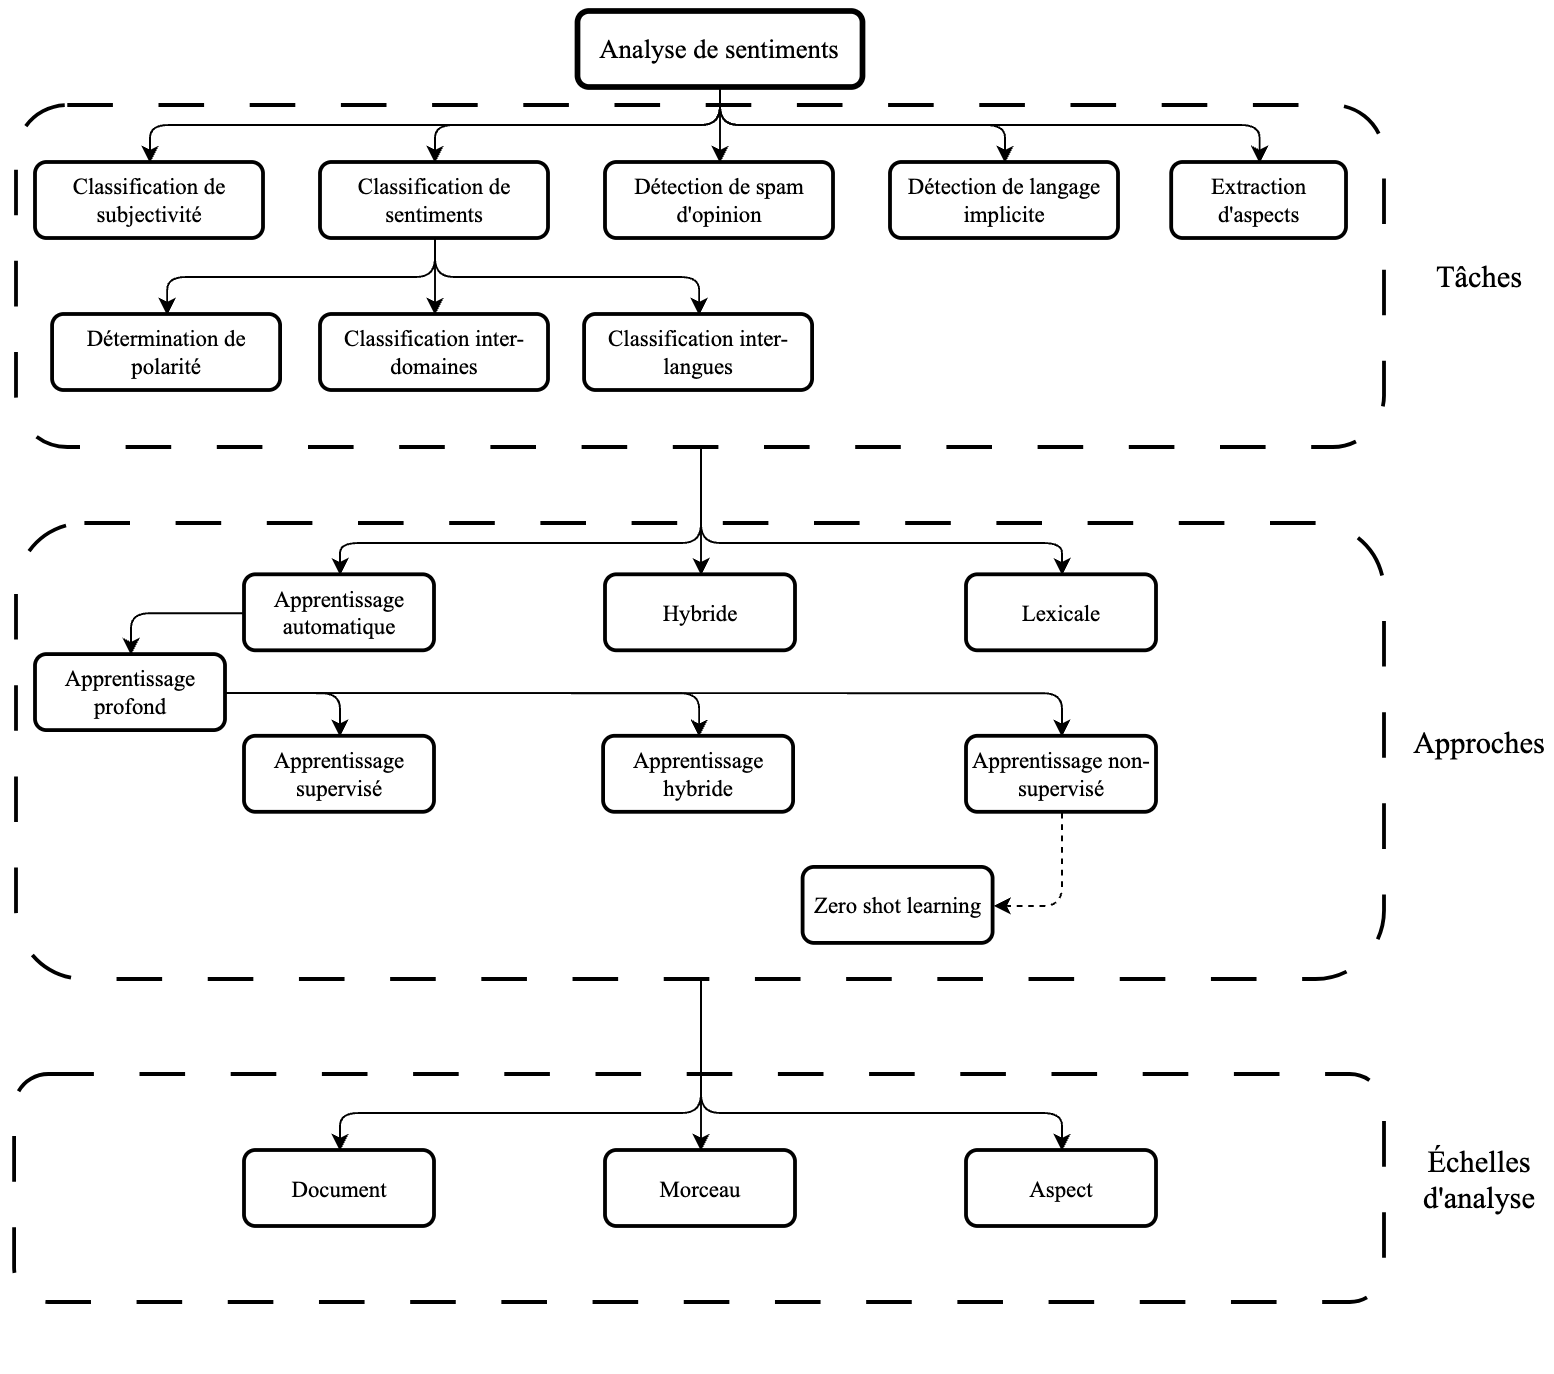
\includegraphics[width=\linewidth]{Images/sentiment_analysis_components}
    \label{fig:SA_apercu}
\end{figure}

La détection de polarité, souvent confondue avec l'ensemble de l'analyse de sentiment, n'est pourtant que l'une des différentes tâches incluses \parencite{cambria17} et celle appliquée ici. Elle fait partie de la classification des sentiments et est traditionnellement définie comme la catégorisation un texte en positif ou négatif \parencite{wang14}. Initialement, cette tâche consistait simplement à détecter, de manière binaire, le sentiment d'un texte. Plus récemment cette tâche a évolué pour mesurer l'intensité du sentiment, c'est-à-dire à quel point est-ce positif ou négatif \parencite{cambria17}. \par 

Le deuxième aspect de l'analyse de sentiment est le choix de l'échelle d'analyse \parencite{liu12}. Typiquement, l'analyse de sentiment peut être réalisée à trois échelles : \textbf{document entier} \parencites{li13, li10, rui13, zhan09}, qui permet d'obtenir le sentiment global; \textbf{morceau par morceau} (mot, phrase, paragraphe, …) \parencites{nguyen18, wilson05, narayanan09, liujun13, yu13}, qui permet une analyse plus fine pour obtenir le sentiment de chaque phrase et \textbf{par aspect}, ce qui permet une analyse du sentiment lié à chaque sujet mentionné. À l'échelle du document entier, l'analyse suppose l'expression d'un seul sentiment de manière cohérente du début à la fin \parencites{pang02, hu11}. \par

Étudier un texte en fonction des différents aspects ou entités présents suppose en fait la succession de deux étapes nécessaires : l'extraction des différents aspects et des phrases concernant chacun d'entre eux, puis l'analyse les sentiments de ces phrases \parencite{liuzhang12}. En fin de compte, ces trois échelles d'analyse répondent à différentes questions et sont complémentaires. \par


Après le choix du type d'analyse et de l'échelle, il reste à choisir parmi les différentes approches méthodologiques. Celles-ci peuvent être résumées en trois catégories : l'approche lexicale, l'approche par apprentissage automatique, et les approches hybrides, mélangeant les deux premières catégories. L'approche lexicale, plus traditionnelle, se base sur un lexique attribuant à chaque mot une valeur positive ou négative. La création de ce lexique est la partie la plus fastidieuse. Une fois le lexique constitué, l'algorithme n'a plus qu'à simplement additionner la valeur des mots connotés positivement ou négativement \parencite{hemmatian19}. Puisque la qualité des résultats d'une approche lexicale dépend du lexique employé, il est nécessaire d'adapter ce lexique au contexte de l'analyse \parencite{ligthart21}, ce qui est chronophage et empêche l'extrapolation des méthodes. Cependant, cette méthode ne nécessite pas de données d'entraînement, à l'inverse des méthodes d'apprentissage automatique. \par

L'approche par apprentissage automatique (ou TALN\footnote{Traitement Automatique du Langage Naturel}), plus récente, est de plus en plus courante et regroupe de nombreuses méthodes. Le principe de base est d'entraîner un algorithme sur des données labellisées, puis d'utiliser cet algorithme sur de nouvelles données afin de leur attribuer des labels et les catégoriser. Les différentes méthodes diffèrent principalement par la technique d'apprentissage. Il existe trois catégories : l'apprentissage supervisé, non supervisé et l'apprentissage hybride \parencite{ligthart21}. Les méthodes de TALN utilisant l'apprentissage supervisé sont supposées apporter de meilleurs résultats, mais sont plus compliquées et coûteuses \parencite{hemmatian19}. Cependant, les méthodes non supervisées gagnent en qualité, notamment grâce à l'Inférence en Langage Naturel et l'apprentissage sans entraînement (zero-shot learning), qui permet de mesurer le lien entre deux textes non familiers, comme un texte et un label. Les méthodes d'apprentissage profond, basées sur les réseaux de neurones, sont de plus en plus proéminentes. \par

\section{Données}
Cette méthodologie est permise par le jeu de données inédit et en accès libre provenant de retours d'expérience d'usagers de l'administration française postés sur le site Je Donne Mon Avis (JDMA). Ces témoignages sont donc en français, modérés, et pour chacun, le sentiment est labellisé par l'auteur. Parmi les variables principales de la base de données, sont aussi incluses l'administration ciblée, la réponse émise, le nombre de personnes ayant signalé avoir vécu une expérience similaire, la satisfaction (binaire) de la réponse de la part de l'auteur et celle des visiteurs du site. \par

Au 2 décembre 2024 inclus, il y avait 65~535 expériences publiées remontant jusqu'au 22 mars 2019. Parmi elles, 77\% expériences sont négatives, 18\% sont positives et 5\% sont neutres (figure~\ref{fig:distrib_ressenti}). 508 structures différentes sont ciblées, parfois plusieurs le sont par une même expérience. Les consulats et ambassades étant inclus dans cette initiative, les expériences peuvent provenir du monde entier. Cependant 89\% d'entre elles proviennent de France. La Direction Interministérielle de la Transformation Publique (DITP) qui gère ce projet garantit une réponse à tout usager, à ce jour 91\% des expériences s'adressant à une structure appartenant au dispositif JDMA ont reçu au moins une réponse. \par

\begin{figure}[ht]
    \centering
    % First figure on the left
    \begin{minipage}[t]{0.48\textwidth}
        \centering
\caption{Distribution des sentiments des usagers.}        
        \includegraphics[width=\linewidth]{Images/distributions_ressenti}
        
        \label{fig:distrib_ressenti}
    \end{minipage}
    \hfill % Horizontal space between the two figures
    % Second figure on the right
    \begin{minipage}[t]{0.48\textwidth}
        \centering
        \caption{Distribution des scores de valence par méthode.}
        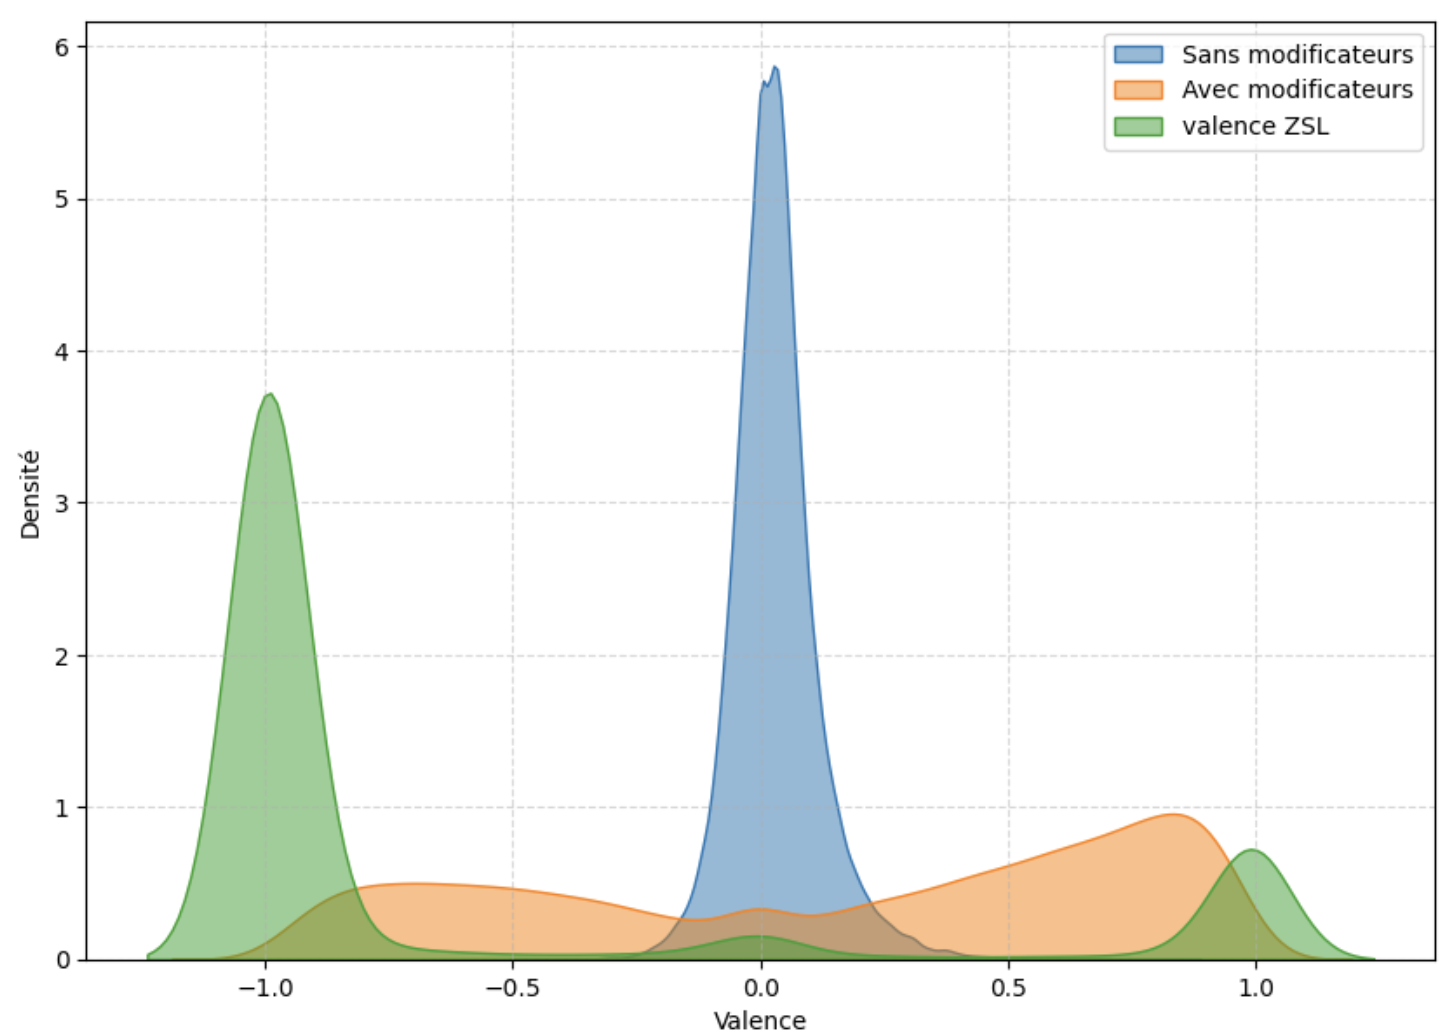
\includegraphics[width=\linewidth]{Images/Distributions}
        
        \label{fig:distributions}
    \end{minipage}
\end{figure}

\section{Sélection de méthode}

Comme mentionné auparavant, les méthodes dictionnaires sont des méthodes nécessitant de la création d'un dictionnaire dans lequel un score positif ou négatif est assigné à chaque mot. Ensuite, ces scores sont additionnés pour créer un score global du sentiment du texte étudié. Les approches avec modificateurs prennent en compte les mots étant neutre par essence comme : "très", "vraiment", etc… mais qui influencent l'intensité d'autres mots en amplifiant leur score. D'autre part, les méthodes d'apprentissage profond et d'inférence se basent sur des réseaux de neurones qui apprennent à partir de données précédemment utilisées. Les méthodes d'inférence se distinguent dans la classification, c'est-à-dire la tâche de catégoriser des données, par leur capacité à utiliser des catégories de labels différentes des données d'entraînement. \par

\subsection{Résultats multiméthodes}
La méthode dictionnaire sans modificateurs (D-SM) nous donne, pour chaque commentaire, les proportions de mots positifs, neutres et négatifs. En soustrayant la proportion de mots négatifs de celle des mots positifs, on obtient un score de valence, c'est-à-dire un score global de sentiment allant de -1 à 1. La méthode avec modificateurs (D-AM), en plus des trois proportions mentionnées de D-SM, nous donne un score de valence global prenant en compte le fait que la majorité des mots utilisés sont neutres, ce score est compris entre -1 et 1. Enfin, la méthode zero-shot learning (ZSL) nous donne la probabilité que chaque valeur de sentiment (positif, neutre, négatif) soit applicable au texte. Comme auparavant, en soustrayant la probabilité que le texte soit négatif de la probabilité qu'il soit positif, nous obtenons encore une fois un score de valence compris entre -1 et 1. \par

Ainsi, nous obtenons trois scores de valence du sentiments compris entre -1 et 1 ; un pour chaque méthode. Or, la distribution de ces scores (figure~\ref{fig:distributions}) nous renseigne sur la validité de leur modèle respectif. Chaque score peut être divisé en trois zones : positive, négative et neutre. Plus un modèle est spécifique, plus la variance dans cette zone est faible. Un modèle spécifique, c'est-à-dire un modèle discriminant la variable mesurée d'autres facteurs, devrait avoir une distribution se rapprochant d'un «\;W\;» : un maximum dans la zone positive, un dans la zone négative et un dans la zone neutre. \textbf{C'est ce que l'on observe pour le ZSL}. \par

En utilisant le score de valence de chaque modèle et en créant des règles nous pouvons répertorier les sentiments. Ici, pour chacun des modèles, si le score est inférieur à $-0,05$ le commentaire est considéré comme négatif, s'il est supérieur à $0,05$ est considéré comme positif et s'il est compris entre les deux, il est considéré comme neutre. En comparant cette répartition issue de chaque modèle avec celle déterminée par les usagers, comme le fait la figure~\ref{fig:heatmaps}, nous pouvons obtenir une mesure de la sensibilité du modèle, c'est à dire sa capacité à reconnaître un label. \textbf{Le modèle de ZSL a le plus haut taux de similarité} avec les usagers avec un score de 90\%. Les scores $F_1$ affichés dans la table~\ref{Fscore} confirment que le ZSL ($F_1 = 0,89$ est plus performant à la fois en précision et en rappel, loin devant le modèle DAM ($F_1 = 0,52$) et le modèle DSM ($F_1 = 0,31$). 
\par 


\begin{figure}[ht]
    \centering
    \caption{Distribution des concordance entre la labellisation de chaque modèle et celle des usagers}
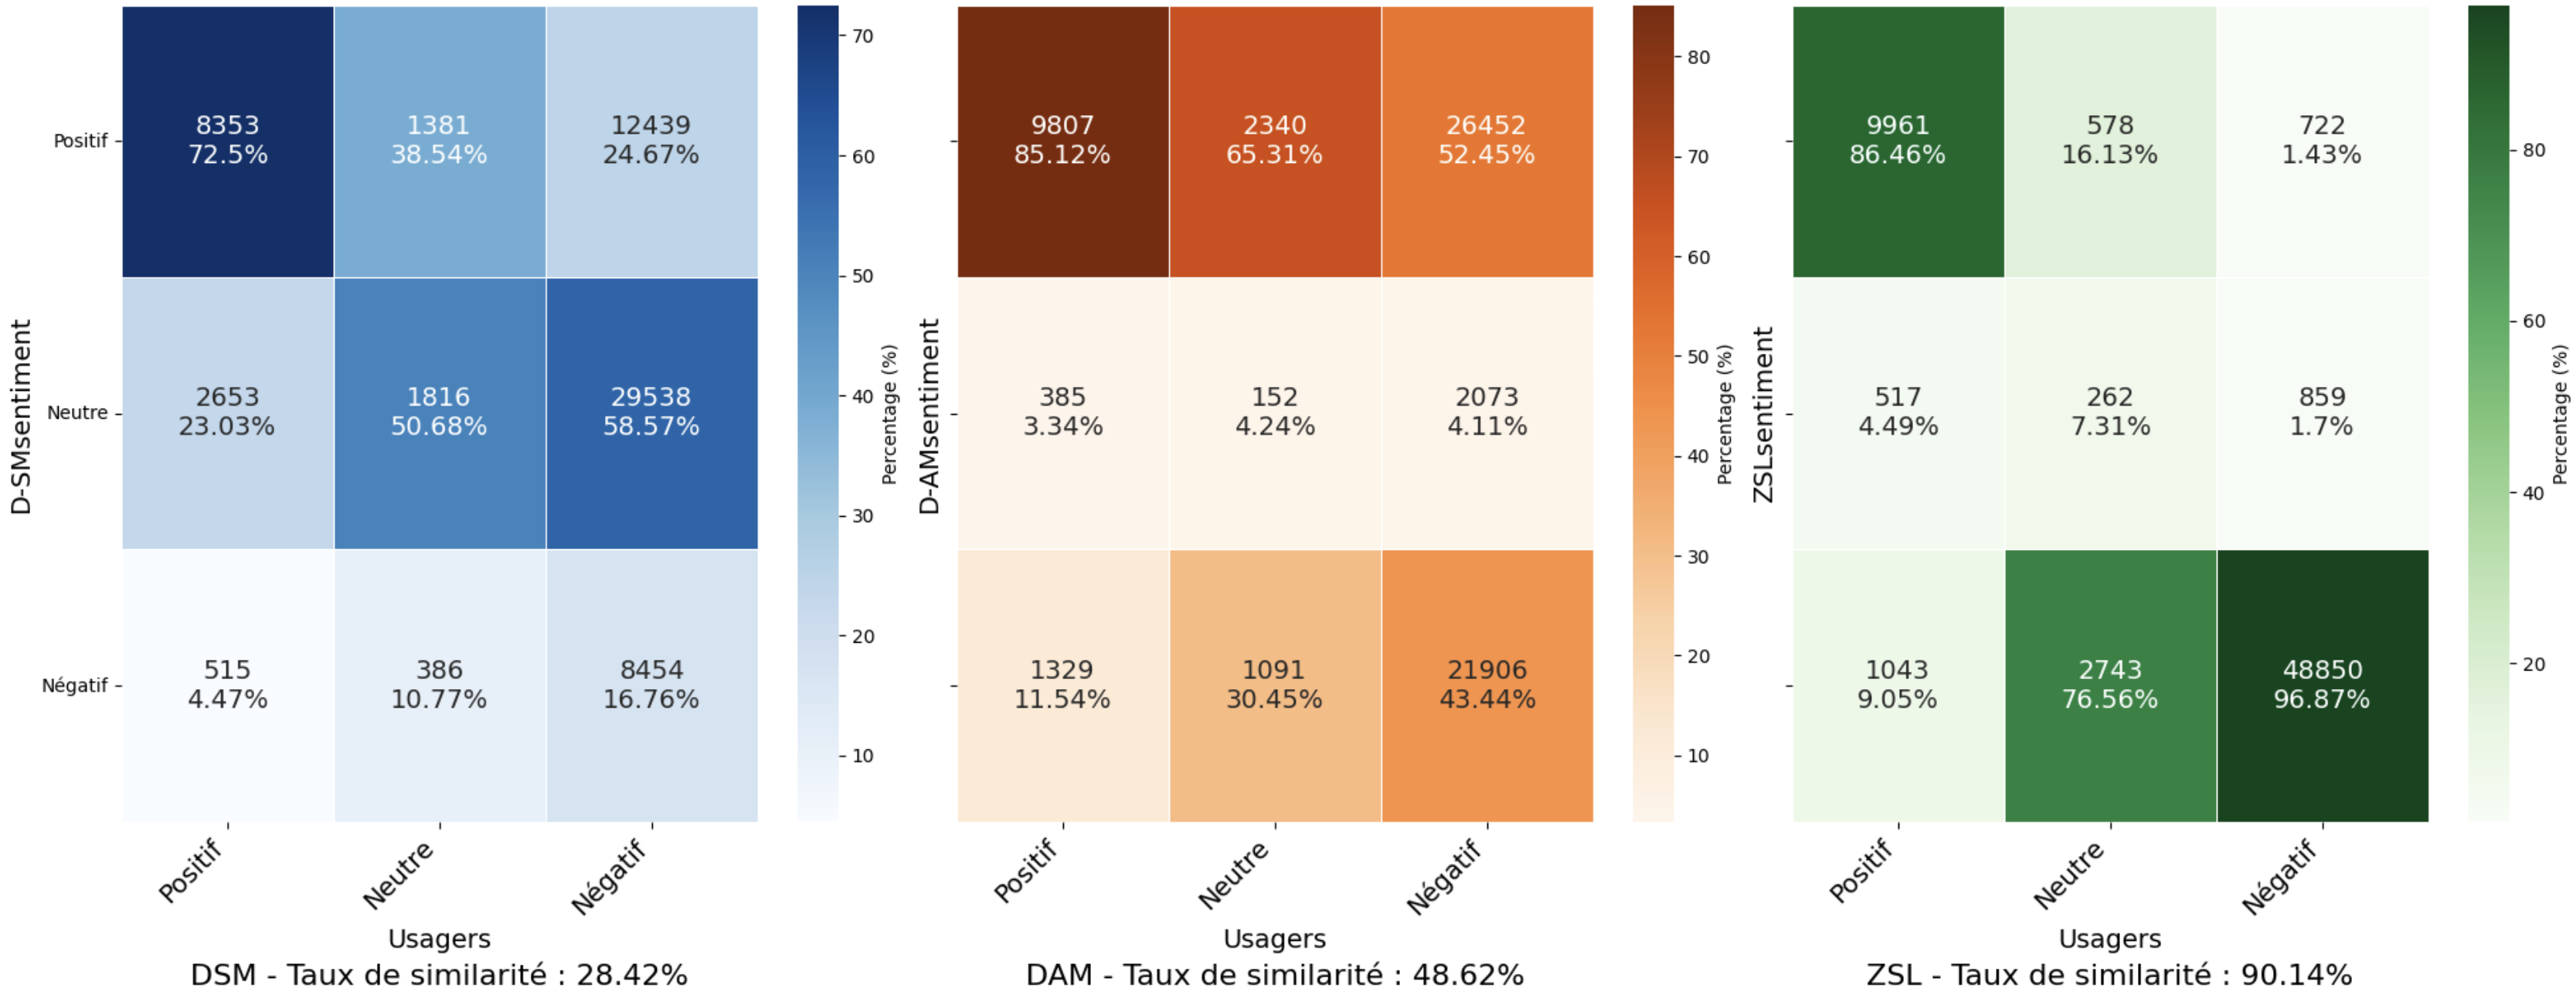
\includegraphics[width=\linewidth]{Images/Heatmaps2}
    
    \label{fig:heatmaps}
\end{figure}





\begin{figure}[ht]
    \centering
    \begin{minipage}{0.4\textwidth}
        \centering
        \captionsetup{width=\linewidth}
        \caption{Scores $F_1$ avec précision et rappel pour chaque modèle.}
        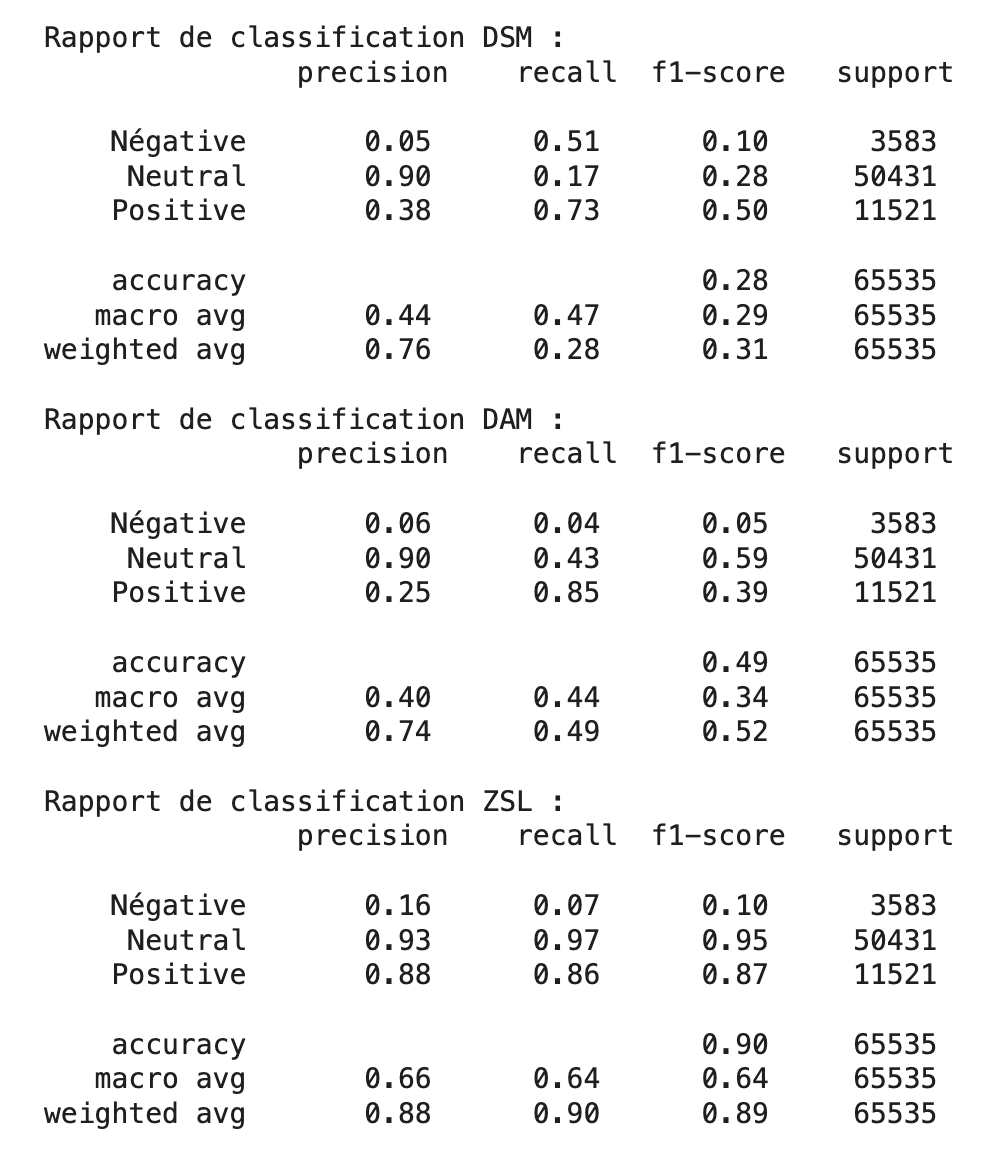
\includegraphics[width=\linewidth]{Images/F_scores}
        
        \label{Fscore}
    \end{minipage}
    \hfill
    \begin{minipage}{0.55\textwidth}
        \centering
                \captionsetup{width=\linewidth}
        \caption{Matrice de corrélations des probabilités de traits.}
        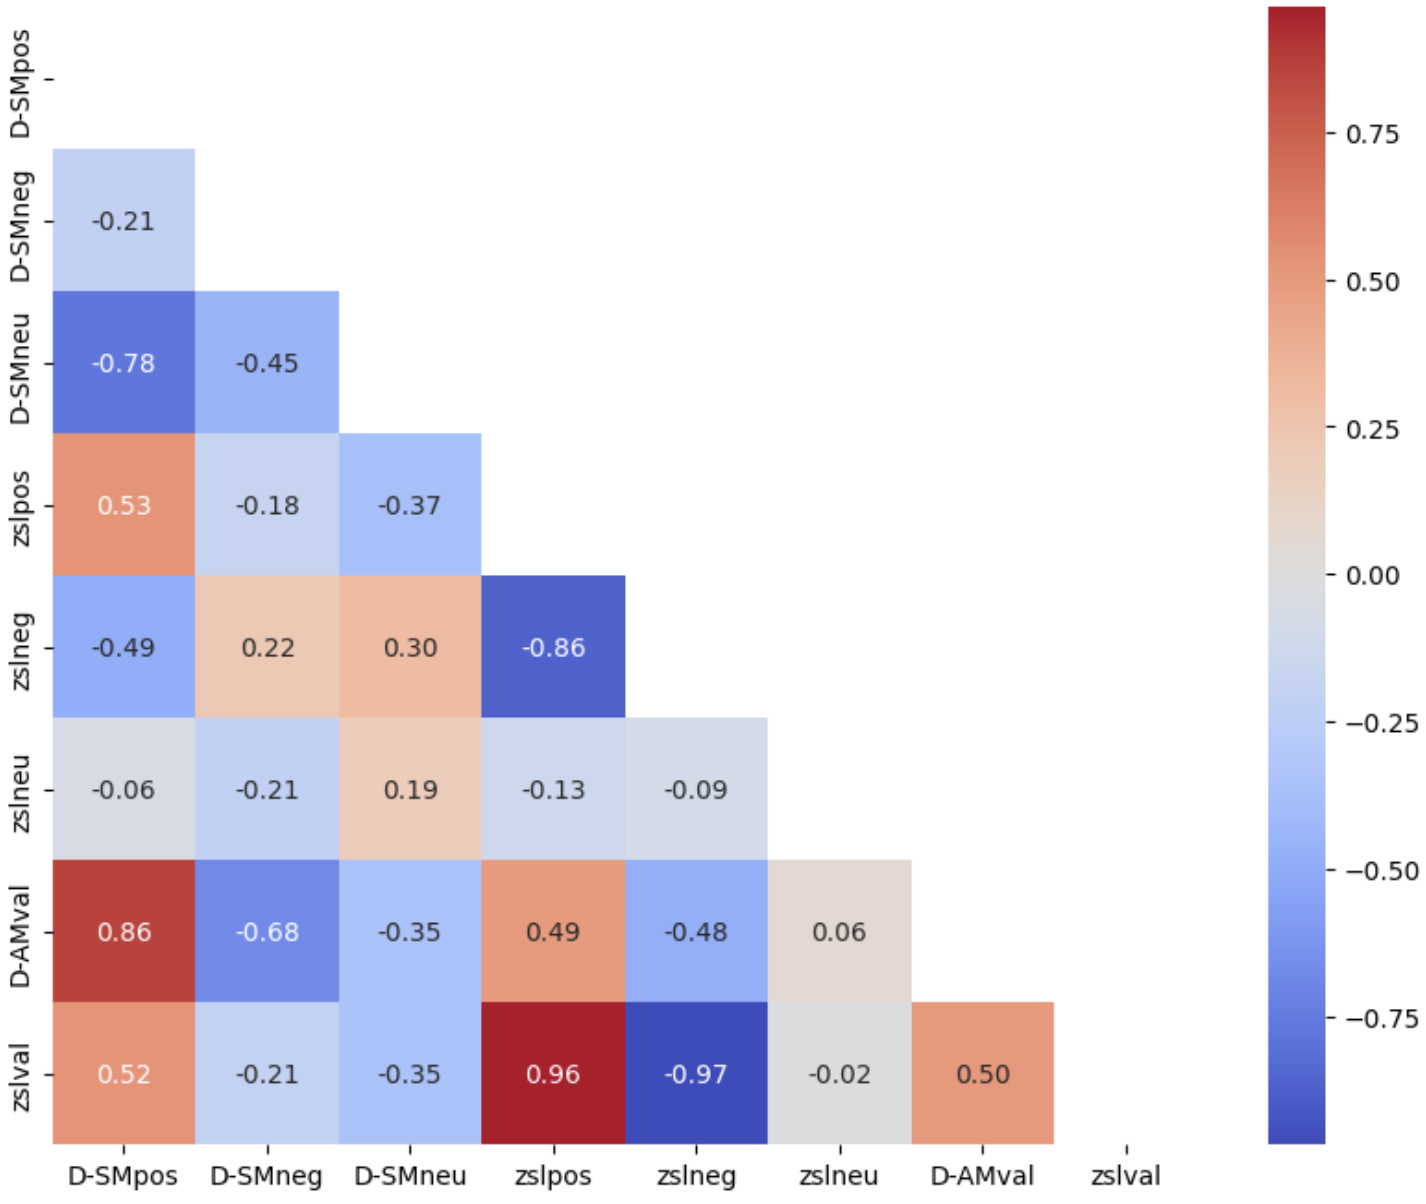
\includegraphics[width=\linewidth]{Images/correlations}

        \label{corr}
    \end{minipage}
\end{figure}



\subsection{Résultats multitraits}



Les modèles D-SM et ZSL nous donnent tous deux une probabilité que chaque commentaire soit positif, négatif ou neutre. Ces six probabilités nous permettent de comparer les résultats. À première vue, la matrice de corrélation (figure~\ref{corr}) nous indique que les scores de sentiment positif sont corrélés entre les deux modèles (r = 0,53).  Cependant, le test de Kolmogorov-Smirnov montre que la distribution de ces deux scores de positivité sont significativement différentes (p-values = 0,0). Il en va de même pour les distributions de scores négatifs et de scores neutres. \par










\end{document}